\section{Entraînement}
    Il a été décidé de faire l'entraînement des réseaux de neurones sur 10 époques, car l'entraînement doit être rapide dans ce contexte.
    
\section{Résultats}

\subsection{Courbes d'apprentissage}

    \begin{figure}[H]
        \centering
        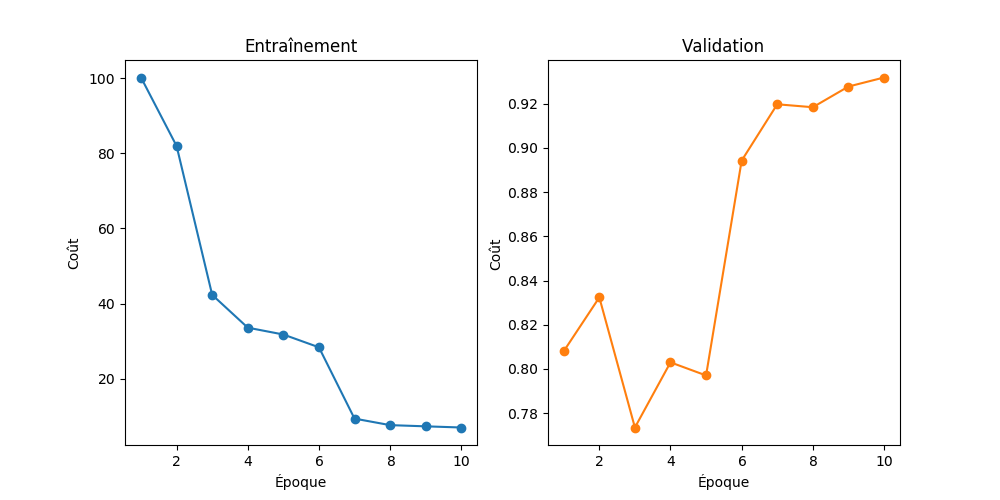
\includegraphics[width=12cm]{images/learning_curves_a.png}
        \caption{Exemple de courbe d'apprentissage du modèle A}
        \label{fig:learning_curves_a}
    \end{figure}

    \begin{figure}[H]
        \centering
        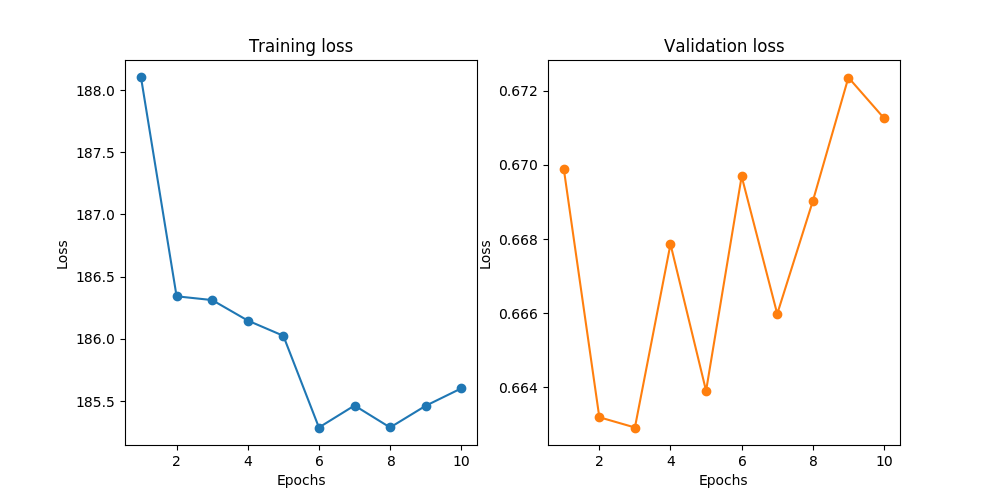
\includegraphics[width=12cm]{images/learning_curves_b.png}
        \caption{Exemple de courbe d'apprentissage du modèle B}
        \label{fig:learning_curves_b}
    \end{figure}

    \begin{figure}[H]
        \centering
        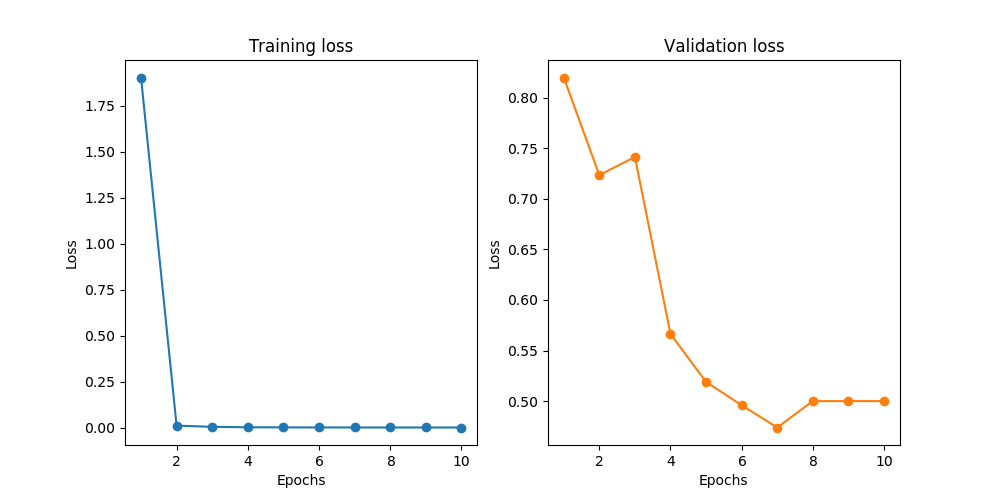
\includegraphics[width=12cm]{images/learning_curves_c.png}
        \caption{Exemple de courbe d'apprentissage du modèle C}
        \label{fig:learning_curves_c}
    \end{figure}

    \begin{figure}[H]
        \centering
        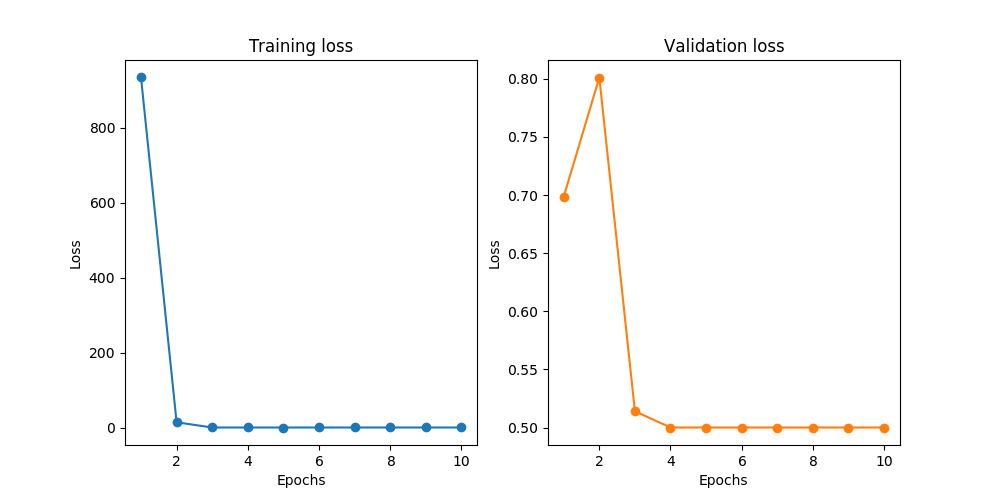
\includegraphics[width=12cm]{images/learning_curves_d.png}
        \caption{Exemple de courbe d'apprentissage du modèle D}
        \label{fig:learning_curves_d}
    \end{figure}

\subsection{Base de données - Tunnel}

\subsubsection{Recherche des hyperparamètres}
    \begin{table}[H]
        \centering
        \caption{Résultat de la recherche des hyperparamètres du modèle A - Tunnel}
        \label{tab:resultat_tunnel_modele_a}
        \begin{tabular}{lllp{3cm}p{3cm}l}
            \midrule
            \# & \(N_A\) & \(N_B\) & Augmentation des données & Métrique de validation & Époque\\
            \midrule\midrule
            1  & 2 & 2 & Non & 0,812 & 10\\
            2  & 2 & 2 & Oui & \\
            3  & 2 & 3 & Non & 0,614 & 1\\
            4  & 2 & 3 & Oui & 0,791 & 7\\
            5  & 4 & 2 & Non & 0,933 & 7\\
            6  & 4 & 2 & Oui & 0,932 & 10\\
            7  & 4 & 3 & Non & 0,930 & 7\\
            \textbf{8}  & \textbf{4} & \textbf{3} & \textbf{Oui} & \textbf{0,936} & \textbf{10}\\
            9  & 8 & 2 & Non & 0,934 & 4\\
            10 & 8 & 2 & Oui & 0,935 & 10\\
            \midrule
        \end{tabular}
    \end{table}

    \begin{table}[H]
        \centering
        \caption{Résultat de la recherche des hyperparamètres du modèle B - Tunnel}
        \label{tab:resultat_tunnel_modele_b}
        \begin{tabular}{lllp{3cm}p{3cm}l}
            \midrule
            \# & \(N_A\) & \(N_B\) & Augmentation des données & Métrique de validation & Époque\\
            \midrule\midrule
            1  & 2 & 2 & Non & 0,612 & 9\\
            2  & 2 & 2 & Oui & 0,673 & 10\\
            3  & 2 & 3 & Non & 0,634 & 1\\
            4  & 2 & 3 & Oui & 0,673 & 6\\
            5  & 4 & 2 & Non & 0,613 & 6\\
            \textbf{6}  & \textbf{4} & \textbf{2} & \textbf{Oui} & \textbf{0,673} & \textbf{2}\\
            7  & 4 & 3 & Non & 0,621 & 4\\
            8  & 4 & 3 & Oui & 0,672 & 9\\
            9  & 8 & 2 & Non & 0,632 & 2\\
            10 & 8 & 2 & Oui & 0,672 & 6\\
            \midrule
        \end{tabular}
    \end{table}

    \begin{table}[H]
        \centering
        \caption{Résultat de la recherche des hyperparamètres du modèle E - Tunnel}
        \label{tab:resultat_tunnel_modele_e}
        \begin{tabular}{lp{3cm}p{3cm}p{3cm}l}
            \midrule
            \# & Entraînement du \text{backend} & Augmentation des données & Métrique de validation & Époque\\
            \midrule\midrule
            \textbf{1} & \textbf{Non} & \textbf{Non} & \textbf{0,931} & \textbf{10}\\
            2 & Non & Oui & 0,926 & 9\\
            3 & Oui & Non & 0,500 & 8\\
            4 & Oui & Oui & 0,500 & 8\\
            \midrule
        \end{tabular}
    \end{table}

\subsubsection{Comparaison entre les modèles}
    \begin{figure}[H]
        \centering
        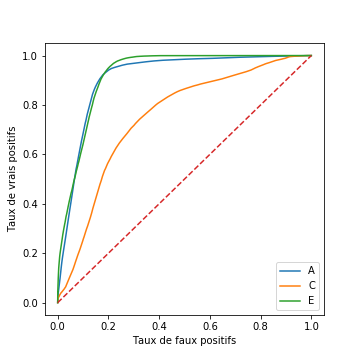
\includegraphics[width=12cm]{images/tunnel_roc.png}
        \caption{Courbes ROC - Tunnel}
        \label{fig:tunnel_roc}
    \end{figure}

    \begin{table}[H]
        \centering
        \caption{Temps d'exécution moyen sur Tesla K20 - Tunnel}
        \label{tab:resultat_tunnel_temps_execution}
        \begin{tabular}{lp{4cm}p{4cm}p{4cm}}
            \midrule
            Modèle & Temps d'exécution moyen de la passe avant (ms) & Temps d'exécution moyen de la passe arrière (ms) & Temps d'exécution total moyen (ms)\\
            \midrule\midrule
            A & 2,93 & 4,75 & 7,68\\
            B & 3,65 & 5,86 & 9,51\\
            E & 3,14 & 2,78 & 5,92\\
            \midrule
        \end{tabular}
    \end{table}

\subsection{Base de données - Faculté de génie}

\subsubsection{Recherche des hyperparamètres}
    \begin{table}[H]
        \centering
        \caption{Résultat de la recherche des hyperparamètres du modèle A - Faculté de génie}
        \label{tab:resultat_corridor_modele_a}
        \begin{tabular}{lllp{3cm}p{3cm}l}
            \midrule
            \# & \(N_A\) & \(N_B\) & Augmentation des données & Métrique de validation & Époque\\
            \midrule\midrule
            1  & 2 & 2 & Non & 0,501 & 1\\
            2  & 2 & 2 & Oui & 0,610 & 7\\
            3  & 2 & 3 & Non & 0,665 & 8\\
            4  & 2 & 3 & Oui & 0,644 & 10\\
            \textbf{5}  & \textbf{4} & \textbf{2} & \textbf{Non} & \textbf{0,678} & \textbf{10}\\
            6  & 4 & 2 & Oui & 0,652 & 10\\
            7  & 4 & 3 & Non & 0,677 & 10\\
            8  & 4 & 3 & Oui & 0,666 & 7\\
            9  & 8 & 2 & Non & 0,667 & 9\\
            10 & 8 & 2 & Oui & 0,672 & 10\\
            \midrule
        \end{tabular}
    \end{table}
    
    \begin{table}[H]
        \centering
        \caption{Résultat de la recherche des hyperparamètres du modèle B - Faculté de génie}
        \label{tab:resultat_corridor_modele_b}
        \begin{tabular}{lllp{3cm}p{3cm}l}
            \midrule
            \# & \(N_A\) & \(N_B\) & Augmentation des données & Métrique de validation & Époque\\
            \midrule\midrule
            1  & 2 & 2 & Non & 0,499 & 7\\
            2  & 2 & 2 & Oui & 0,503 & 5\\
            3  & 2 & 3 & Non & 0,499 & 10\\
            4  & 2 & 3 & Oui & 0,502 & 4\\
            \textbf{5}  & \textbf{4} & \textbf{2} & \textbf{Non} & \textbf{0,511} & \textbf{1}\\
            6  & 4 & 2 & Oui & 0,501 & 10\\
            7  & 4 & 3 & Non & 0,501 & 8\\
            8  & 4 & 3 & Oui & 0,500 & 2\\
            9  & 8 & 2 & Non & 0,499 & 1\\
            10 & 8 & 2 & Oui & 0,501 & 10\\
            \midrule
        \end{tabular}
    \end{table}
    
    \begin{table}[H]
        \centering
        \caption{Résultat de la recherche des hyperparamètres du modèle E - Faculté de génie}
        \label{tab:resultat_corridor_modele_e}
        \begin{tabular}{lp{3cm}p{3cm}p{3cm}l}
            \midrule
            \# & Entraînement du \text{backend} & Augmentation des données & Métrique de validation & Époque\\
            \midrule\midrule
            \textbf{1} & \textbf{Non} & \textbf{Non} & \textbf{0,719} & \textbf{10}\\
            2 & Non & Oui & 0,699 & 7\\
            3 & Oui & Non & 0,500 & 10\\
            4 & Oui & Oui & 0,500 & 10\\
            \midrule
        \end{tabular}
    \end{table}

\subsubsection{Comparaison entre les modèles}
    \begin{figure}[H]
        \centering
        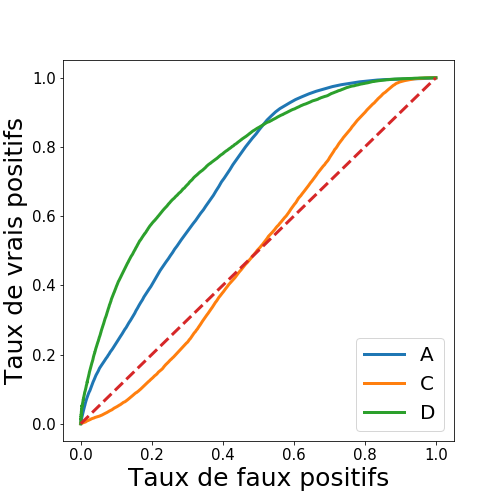
\includegraphics[width=12cm]{images/corridor_roc.png}
        \caption{Courbes ROC - Faculté de génie}
        \label{fig:corridor_roc}
    \end{figure}

    \begin{table}[H]
        \centering
        \caption{Temps d'exécution moyen sur Tesla K20 - Faculté de génie}
        \label{tab:resultat_corridor_temps_execution}
        \begin{tabular}{lp{4cm}p{4cm}p{4cm}}
            \midrule
            Modèle & Temps d'exécution moyen de la passe avant (ms) & Temps d'exécution moyen de la passe arrière (ms) & Temps d'exécution total moyen (ms)\\
            \midrule\midrule
            A & 3,08 & 4,22 & 7,30\\
            B & 3,65 & 5,86 & 9,51\\
            E & 3,14 & 2,78 & 5,92\\
            \midrule
        \end{tabular}
    \end{table}

\subsection{Analyse générale}
    